\clearpage
\subsection{Procedure Call} % (fold)
\label{sub:procedure call}

A Procedure Call is a kind of \nameref{sec:program-creation-statement} that instructs the computer to run the code in a \nameref{sub:procedure}. If the Procedure requires some data to work with, then this data is passed to the Procedure as part of the Procedure Call. The Procedure's name is used to identify the Procedure to call.

\begin{figure}[h]
   \centering
   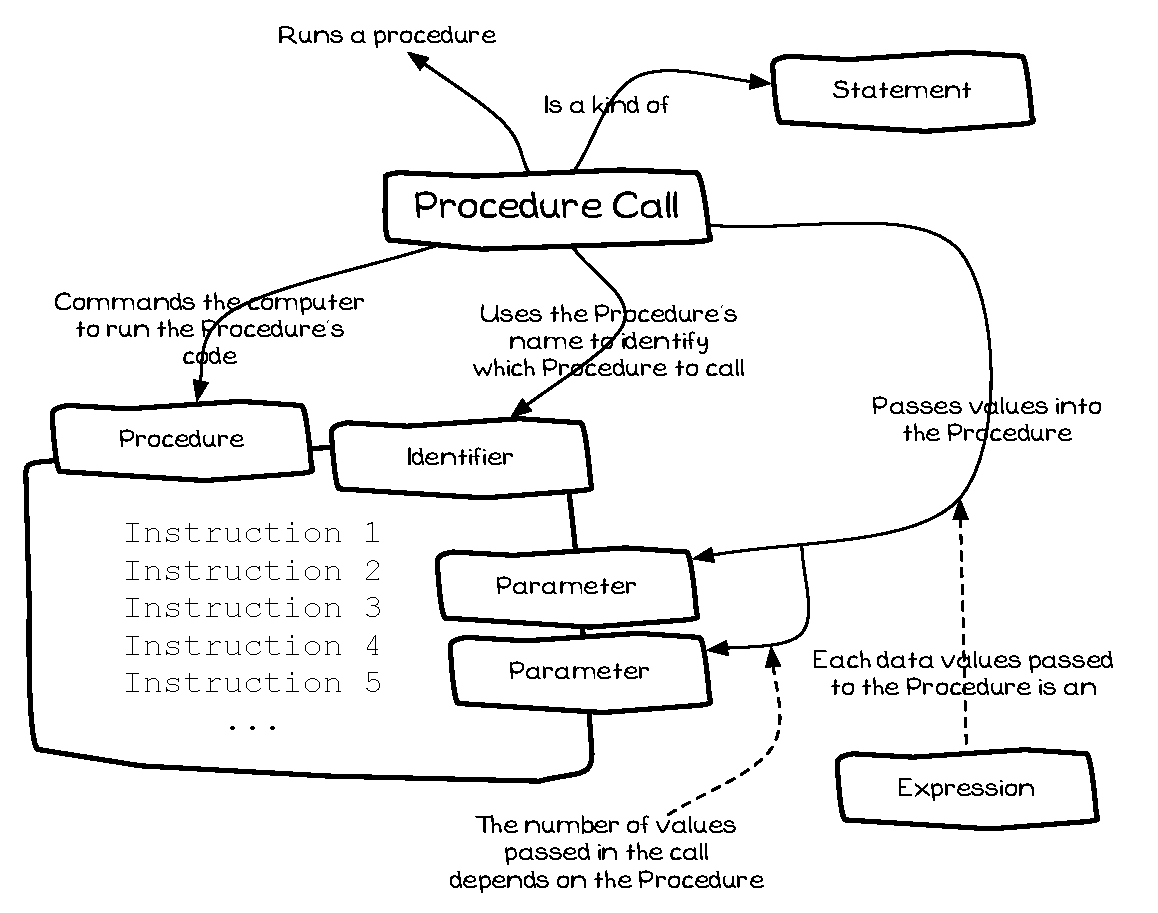
\includegraphics[width=\textwidth]{./topics/program-creation/diagrams/ProcedureCall} 
   \caption[Procedure Call Concept Diagram]{A Procedure Calls runs a Procedure, passing in values for the procedure to use}
   \label{fig:program-creation-procedure call}
\end{figure}


\mynote{
\begin{itemize}
  \item Figure \ref{fig:program-creation-procedure call} shows the concepts related to the Procedure Call.
  \item A Procedure Call is an instruction to execute a Procedure.
  \item The \nameref{sub:identifier} indicates the \nameref{sub:procedure} to call.
  \item Data values passed to the Procedure are \nameref{sub:expression}s.
  \item When the Procedure's task is complete the program continues with the next \nameref{sec:program-creation-statement}.
\end{itemize}
}

% section program (end)